\documentclass[areasetadvanced]{scrartcl}

\usepackage[utf8]{inputenc}
\usepackage[T2A]{fontenc}
\usepackage[english,russian]{babel}

\usepackage[footskip=1cm,left=25mm, right=15mm, top=20mm, bottom=20mm]{geometry}
\usepackage{setspace}
\usepackage{amsmath, amssymb} 
\usepackage{graphicx}
\usepackage{tikz}
\usetikzlibrary{arrows.meta}
\usepackage{float}
\usepackage{dashrule}
\usepackage{fancyhdr} 
\usepackage{hyperref} 
\usepackage{parskip}
\usepackage{textcomp, enumitem}
\usepackage{indentfirst}
\usepackage{graphicx}
\usepackage{algorithm}
\usepackage{algpseudocode}
\usepackage{array} 
\usepackage{geometry}
\usepackage{afterpage}
\usepackage{minted}
\setcounter{secnumdepth}{3} 
\setcounter{tocdepth}{3}    
\usepackage{listings} 

\tikzstyle{block} = [rectangle, rounded corners, minimum width=3cm, minimum height=1cm, text centered, draw=black, fill=lightgray]

\setkomafont{sectioning}{\normalfont\bfseries} 
\setkomafont{section}{\normalfont\Large\bfseries}
\setkomafont{subsection}{\normalfont\large\bfseries}
\setkomafont{subsubsection}{\normalfont\large\bfseries}
\setkomafont{paragraph}{\normalfont\large\bfseries} 

\lstset{
  language=Haskell,
  basicstyle=\ttfamily\small,
  keywordstyle=\color{blue}\bfseries,
  stringstyle=\color{red},
  commentstyle=\color{green!70!black},
  numbers=left,
  numberstyle=\tiny,
  stepnumber=1,
  numbersep=10pt,
  showstringspaces=false,
  breaklines=true,
  frame=single
}
\setlength{\parindent}{1.25cm}
\setcounter{tocdepth}{3}
\begin{document}
\sloppy
	\thispagestyle{empty}
	\begin{center}
		\large{МИНОБРНАУКИ РОССИИ} \par
		\vspace{0.3cm}
		\normalsize
		{ФЕДЕРАЛЬНОЕ ГОСУДАРСТВЕННОЕ АВТОНОМНОЕ ОБРАЗОВАТЕЛЬНОЕ УЧРЕЖДЕНИЕ ВЫСШЕГО ОБРАЗОВАНИЯ} \par
		\vspace{0.3cm}
		\textbf{\guillemotleft САНКТ-ПЕТЕРБУРГСКИЙ ПОЛИТЕХНИЧЕСКИЙ}
		\textbf{УНИВЕРСИТЕТ ПЕТРА ВЕЛИКОГО\guillemotright} \par
		\vspace{0.3cm}
		{Институт компьютерных наук и кибербезопасности}\par
		{Высшая школа технологий искусственного интеллекта}\par
	\end{center}
	\vfill
	\begin{center}
		{\large Отчёт по дисциплине \guillemotleft Алгоритмические основы компьютерной графики\guillemotright}\par
		{\huge   Лабораторная работа №3
		
		\guillemotleft Анимация сцены\guillemotright}\par
            {\huge Вариант: \textbf{Кипение воды в чайнике (фаза 4)}}
         
	\end{center}
	\vfill
	\begin{flushleft}
		Студент: \hspace{1.8cm} \rule[0pt]{2.5cm}{0.5pt}\hfill Салимли Айзек Мухтар Оглы\par
		\vspace{1.5cm}
		Преподаватель: \hspace{0.55cm} \rule[0pt]{2.5cm}{0.5pt}\hfill  Курочкин Михаил Александрович
	\end{flushleft}
	\vspace{0.5cm}
	\begin{flushright}
		\guillemotleft \rule[0pt]{0.8cm}{0.5pt}\guillemotright \rule[0pt]{2cm}{0.5pt} 20\rule[0pt]{0.5cm}{0.5pt} г.
	\end{flushright}
	\vfill
	\begin{center}
		Санкт-Петербург, 2025
	\end{center}
	\newpage
	\tableofcontents
	\newpage
\section*{Введение}
	\addcontentsline{toc}{section}{Введение}

Компьютерная графика — это раздел информатики, предметом которого является создание и обработка изображений с помощью компьютерных технологий. Одним из распространённых направлений является компьютерная анимация. Она позволяет создавать движущиеся изображения с помощью графических изображений. С помощью средств компьютерной графики можно моделировать визуально любой физический процесс. В настоящее время есть несколько видов анимации:
\begin{itemize}
    \item покадровая анимация;
    \item анимация записи движения;
    \item процедурная анимация;
    \item анимация с помощью программных продуктов.
\end{itemize}

Процедурная анимация — это вид компьютерной анимации, который автоматически генерирует анимацию в реальном времени согласно установленным правилам, законам и ограничениям.

Цель данной работы — создание визуализации реального физического процесса, который представлен в видеоролике, фиксирующем процесс кипения чайника.

Основные характеристики визуализации реального физического процесса включают:
\begin{itemize}
    \item временную протяжённость: процесс кипения воды изменяется во времени, что требует создания анимации;
    \item статические и динамические элементы: в данном процессе присутствуют как неизменные элементы, так и те, которые меняют свою форму и положение.
\end{itemize}
\newpage
\section{Постановка задачи}
Требуедеоролик физического процесса - кипение чайника, фаза 4.
\begin{itemize}
    \item проанализировать видеоролик, выделить особенности в физическом процессе;
    \item разработать метод визуализации;
    \item реализовать визуализацию процесса при помощи графической библиотеки.
\end{itemize}
Скриншот (кадр) из видеоролика представлен на Рис.\ref{fig:first}.
\begin{figure}[H]
    \centering
    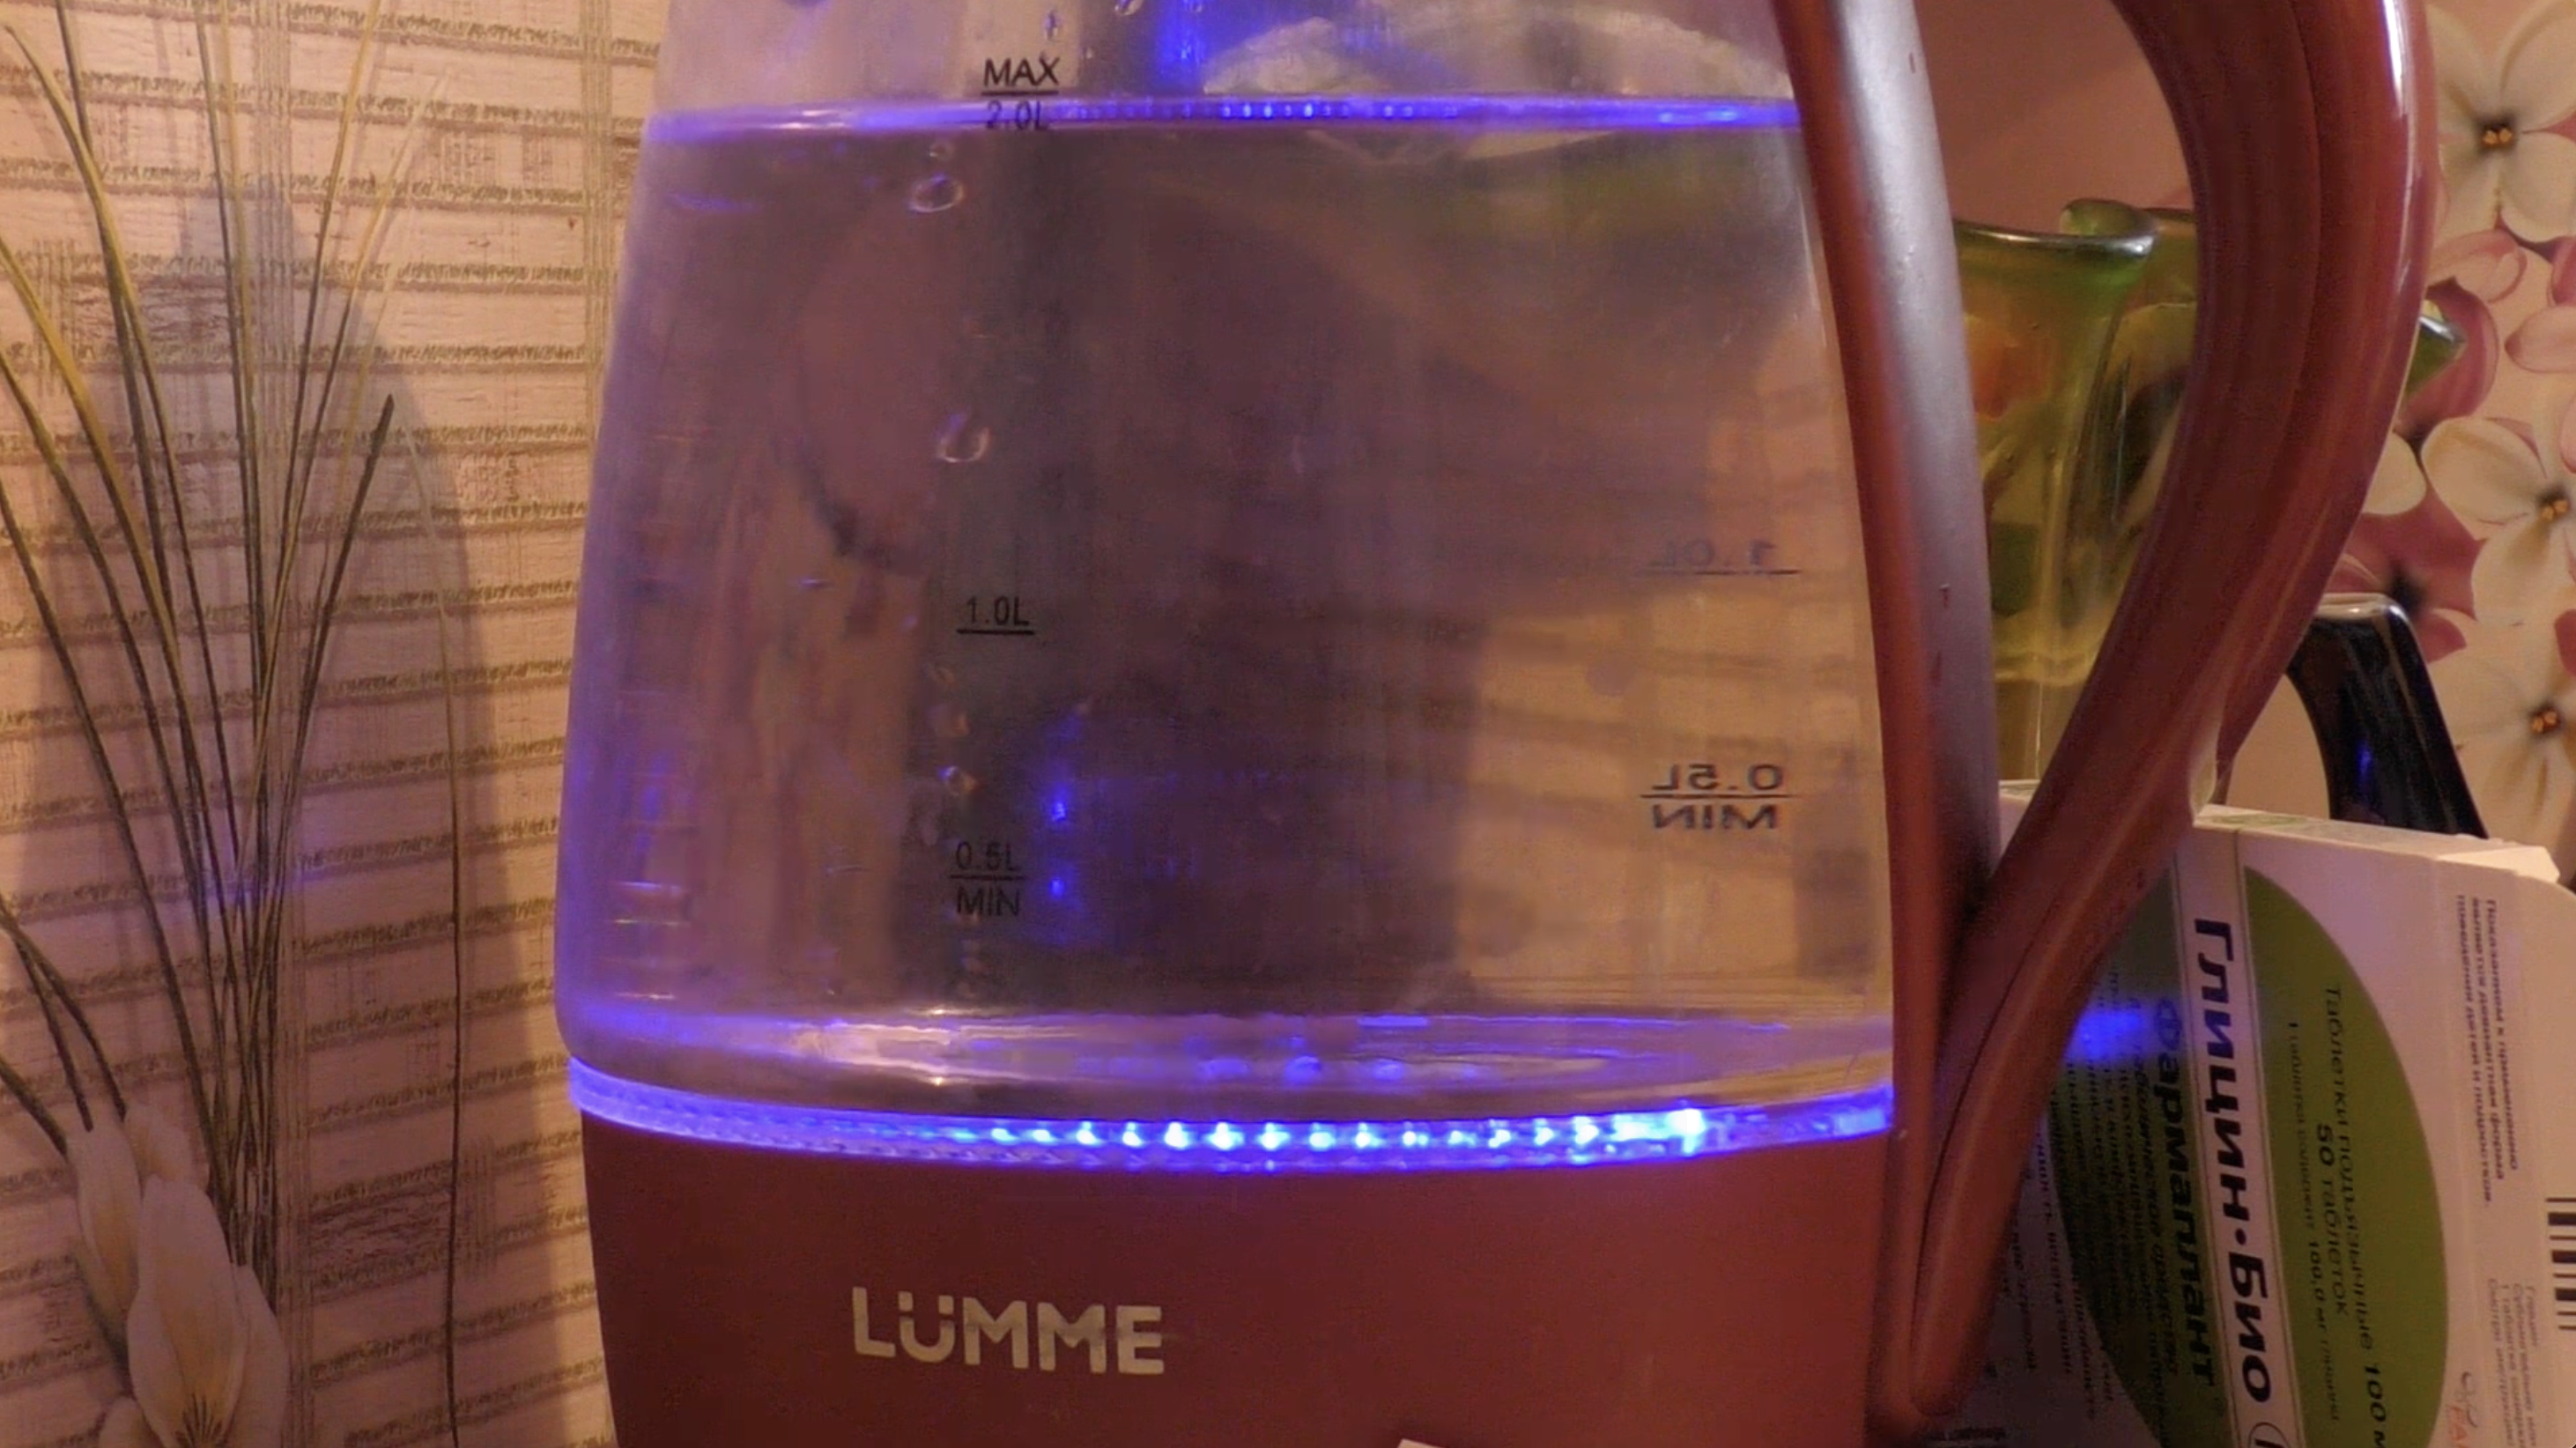
\includegraphics[width=0.5\textwidth]{images/image.png}
    \caption{Скриншот (кадр) из видеоролика}
    \label{fig:first}
\end{figure}

\newpage
\section{Описание физического процесса}
Физический процесс можно разделить на статическую и динамическую части.\\

\textbf{Статическая часть:}
\begin{enumerate}
    \item \textbf{Электрический чайник (на переднем плане)}\\
    Чайник преимущественно красного цвета с прозрачным резервуаром для воды. На боковой стороне резервуара есть отметки, указывающие уровень воды («2,0 л», «1,0 л», «0,5 л», «MIN»). Вдоль основания чайника проходит синяя светодиодная лента. Ручка тоже красная, сделана из пластика.
    \item \textbf{Фон}\\
    На фоне узорчатые обои с цветочным рисунком. Преобладающие цвета — бежевый или светло-коричневый с более тёмными коричневыми цветочными узорами.\\
    Справа от чайника видна упаковка глицина. А между спинкой чайника и ручкой видна ваза.
    \item \textbf{Освещение и тени}\\
    Освещение в сцене мягкое и рассеянное, создающее тени. Синие светодиоды на чайнике создают лёгкое свечение на переднем плане, контрастирующее с более тёплыми тонами фона.
\end{enumerate}

\textbf{Динамическая часть:}\\
Для описания нужно предположить реальные размеры предметов на видео. Если на видео представлен стандартный чайник, то 100 пикселям на этом видео соответствует примерно 1.5 см.

\begin{enumerate}
    \item \textbf{Кипение воды:}\\
    Внутри прозрачного корпуса чайника происходит интенсивное кипение. Мелкие пузыри формируются на дне, быстро растут при подъёме и лопаются у поверхности воды. Движение жидкости хаотично, с явными конвекционными потоками. Высота зоны кипения составляет около \textbf{25 см}, максимальный диаметр пузырей — до \textbf{0.5 см}. Делятся эти пузырьки на две части:
    \begin{enumerate}
        \item[(a)] \textbf{Пузыри основного кипения.}\\
        Радиус пузырьков составляет \textbf{0.08--0.19 см}\footnote{8–19 пикселей при масштабе 100 px = 1 см}, 
        скорость подъёма — \textbf{4–7 см/с}\footnote{0.4–0.7 px/мс}.  
        Горизонтальные колебания имеют амплитуду до \textbf{0.26 см} (26 px).  
        Время жизни одного пузырька — около \textbf{1 с}; в секунду возникает порядка \textbf{250} пузырьков.
    \end{enumerate}
    
\end{enumerate}
Размер пузырьков меняется по ходу движения как в большую, так и в меньшую сторону. При этом при таком движении блики в них тоже изменяют свое положение.

Плотность пузырьков примерно \textbf{10 пузырьков на 10$\times$10 см}.

\begin{enumerate}
    \setcounter{enumi}{0}
    \item[(b)] \textbf{Пузыри рядом с основным кипением.}\\
    Некоторые пузырьки с основного потока попадают в правую часть чайника, где движутся не так активно и намного более хаотично, без явной траектории.\\
    Выглядят пузырьки там так же, но их плотность меньше, около \textbf{7--10 пузырьков на 10$\times$10 см}.
\end{enumerate}

2. \textbf{Турбулентность и конвекция:}\\
Турбулентность проявляется в виде случайных завихрений и колебаний потоков воды. Конвекционные ячейки создают направленное движение жидкости вверх-вниз. Скорость пузырей достигает 120 пикселей/секунду, что определяется тепловым расширением и гидродинамическим сопротивлением.

\textbf{1. Параметры кипения:}
\begin{itemize}
    \item Высота зоны кипения: 2.5 см.
    \item Диапазон диаметров пузырей: [0.05, 0.3] см.
    \item Цвет воды: RGB(180, 200, 255) — голубой оттенок из-за подсветки.
    \item Прозрачность: $\alpha = 0.7$ — частичная видимость внутренней структуры.
\end{itemize}

\textbf{2. Физические параметры:}
\begin{align*}
    &\text{Гравитация } g = 9.8~\text{м/с}^2 \\
    &\text{Турбулентность } \tau = 0.15 \\
    &\text{Базовая скорость пузырей } v_0 = 120~\text{пикс/сек} \\
    &\text{Коэффициент сопротивления } k = 0.6 \\
    &\text{Частота образования пузырей } f = 50~\text{пузырей/сек} \\
\end{align*}

\begin{itemize}
    \item Гравитация $g = 9.8~\text{м/с}^2$\\
    \textit{Обоснование:} стандартное ускорение свободного падения для реалистичной модели.
    \item Турбулентность $\tau = 0.15$\\
    \textit{Обоснование:} небольшое значение для имитации начала кипения.
    \item Сопротивление $k = 0.6$\\
    \textit{Обоснование:} учитывает трение между водой и стенками чайника.
    \item Частота $f = 50~\text{пузырей/сек}$\\
    \textit{Обоснование:} соответствует интенсивности кипения при нагреве.
\end{itemize}

\newpage
\subsection{Визуальные параметры}
\begin{itemize}
    \item Цвет подсветки: RGB(0, 0, 255)
    \textit{Обоснование:} синий светодиодный свет создает холодный эффект.
    \item Размер пузырей: $r \in [0.08, 0.19]$ см
    \textit{Обоснование:} прогрессивное увеличение при подъеме.
    \item Размытие Гаусса: ядро $\,\sigma\!=\!1.5$
    \textit{Обоснование:} для плавного перехода между пузырями.
    \item Отражение света: коэффициент 0.4
    \textit{Обоснование:} имитация прозрачности воды и стекла.
    \item Основная непрозрачность стеклянной оболочки: $\alpha_{\text{glass}} = 0.35$
    \item Прозрачность воды: $\alpha_{\text{water}} = 0.7$
\end{itemize}

\newpage
\subsection{Динамика пузырей}
Путем подбора были выбраны следующие уравнения для описания движения пузырьков.

\begin{itemize}
    \item \textbf{Основные пузырьки:}
    \begin{itemize}
        \item[] Уравнение траектории:
        \[
        \begin{cases}
            x(t) = x_0 + A \cdot \sin\left(\pi \cdot \frac{t}{t_{\text{peak}}}\right), \\\\
            y(t) = y_0 - v \cdot t,
        \end{cases}
        \]
        где:
        \begin{itemize}
            \item[] $A = 1.2 \cdot 150$ — амплитуда
            \item[] $v$ — скорость
            \item[] $t_{\text{peak}}$ — время достижения пика
        \end{itemize}
    \end{itemize}

    \item \textbf{Дополнительные пузырьки:}
    \begin{itemize}
        \item Хаотичное движение в прямоугольной области 120 $\times$ 60 пикселей
        \item Синусоидальные колебания с частотой 20 -- 25 Гц
    \end{itemize}
    \item Динамическое изменение размера пузырьков с амплитудой 30\%
    \item Анимация бликов:
    \begin{itemize}
        \item Блик смещается по синусоиде с частотой 1.8 Гц
        \item Яркость зависит от фазы:
        \[
            \text{opacity} = 80 \times (0.8 + 0.2 \sin(0.6 t))
        \]
    \end{itemize}
    \item Прозрачность пузырька колеблется: 
    $\alpha(t)=\alpha_0\!\cdot\!\bigl(0.8+0.2\,\sin(0.6\,t+\varphi)\bigr)$.
    \item Каждый пузырь содержит \emph{двойной блик}: 
    главный радиусом $0.45\,r$ и вторичный $0.20\,r$
    \item Края пузыря дополнительно размываются фильтром 
    \textit{GaussianBlur($\sigma =\!1.5$)}.
    \end{itemize}

\newpage
\section{Описание реализации визуализации кипения воды в чайнике}
Данная визуализация реализована на языке Python с использованием библиотеки PIL/Pillow для обработки изображений и генерации анимации. Программа создает реалистичный эффект кипения, моделируя два типа пузырьков: основные (идущие с дна чайника) и вторичные (в правой части чайника). Для повышения физической достоверности учитывается влияние температуры на скорость испарения и динамику пузырьков.
\subsection{Структура программы}
\begin{itemize}
    \item Основные пузырьки генерируются в диапазоне координат:
    \begin{itemize}
        \item $X \in [830, 1750]$
        \item $Y \in [560, 1250]$
    \end{itemize}
    \item Дополнительные пузырьки появляются в зоне:
    \begin{itemize}
        \item $X \in [1300, 1600]$
        \item $Y \in [120, 700]$
    \end{itemize}
\end{itemize}

Эти параметры подобраны опытным путем, чтобы задать границы стенок чайника.

\begin{itemize}
    \item Каждый пузырек имеет уникальные параметры:
    \begin{itemize}
        \item Случайная начальная фаза (\textit{phase}) для асинхронности движения
        \item Радиус пузырька выбирается случайно из диапазона 8–19 px.
        \item Генерируется \textbf{250} основных и \textbf{40} дополнительных пузырей на каждые 60 кадров.
        \item Скорость:
        \begin{itemize}
            \item 0.3 -- 0.5 пикселей/мс для основных пузырьков
            \item 0.01 -- 0.05 пикселей/мс для дополнительных пузырьков
        \end{itemize}
        \item Частота изменения размера: 0.2 -- 0.6 Гц с затуханием по мере подъема
    \end{itemize}
\end{itemize}

\textbf{2. Траектории движения}

\begin{itemize}
    \item \textbf{Основные пузырьки:}
    \begin{itemize}
        \item Движение по модифицированной параболе с кривизной 1.2
        \item Горизонтальные колебания с амплитудой до 150 пикселей
        \item Время жизни: 1 секунда ($\approx$ 50 кадров при 50 FPS)
    \end{itemize}
    \item \textbf{Дополнительные пузырьки:}
    \begin{itemize}
        \item Хаотичное движение в прямоугольной области 120 $\times$ 60 пикселей
        \item Синусоидальные колебания с частотой 20 -- 25 Гц
    \end{itemize}
    \item Динамическое изменение размера пузырьков с амплитудой 30\%
    \item Анимация бликов:
    \begin{itemize}
        \item Блик смещается по синусоиде с частотой 1.8 Гц
        \item Яркость зависит от фазы:
        \[
            \text{opacity} = 80 \times (0.8 + 0.2 \sin(0.6 t))
        \]
    \end{itemize}
    \item Прозрачность пузырьков: базовое значение 80 (из 255) с градиентом по краям
    \item Рефракция света на границе пузырька с водой
    \end{itemize}

\textbf{4. Маскирование}
\begin{itemize}
    \item Пузырики отображаются только внутри полигона с координатами:
    \[
        (430, 780),\ (510, 10),\ (1300, 10),\ (1370, 870)
    \]
    \item Реализована точная проверка принадлежности точки полигону методом лучей
    \item Постепенное исчезновение при приближении к границе
\end{itemize}

\newpage
\section{Результаты работы программы}
На Рис.\ref{fig:result} представлен результат визуализации кипения воды в чайнике.
На Рис.\ref{fig:base} представлен базовый кадр.
\begin{figure}[H]
    \centering
    \begin{minipage}{0.48\textwidth}
        \centering
        \includegraphics[width=\linewidth]{images/result.png}
        \caption{Результаты визуализации}
        \label{fig:result}
    \end{minipage}\hfill
    \begin{minipage}{0.48\textwidth}
        \centering
        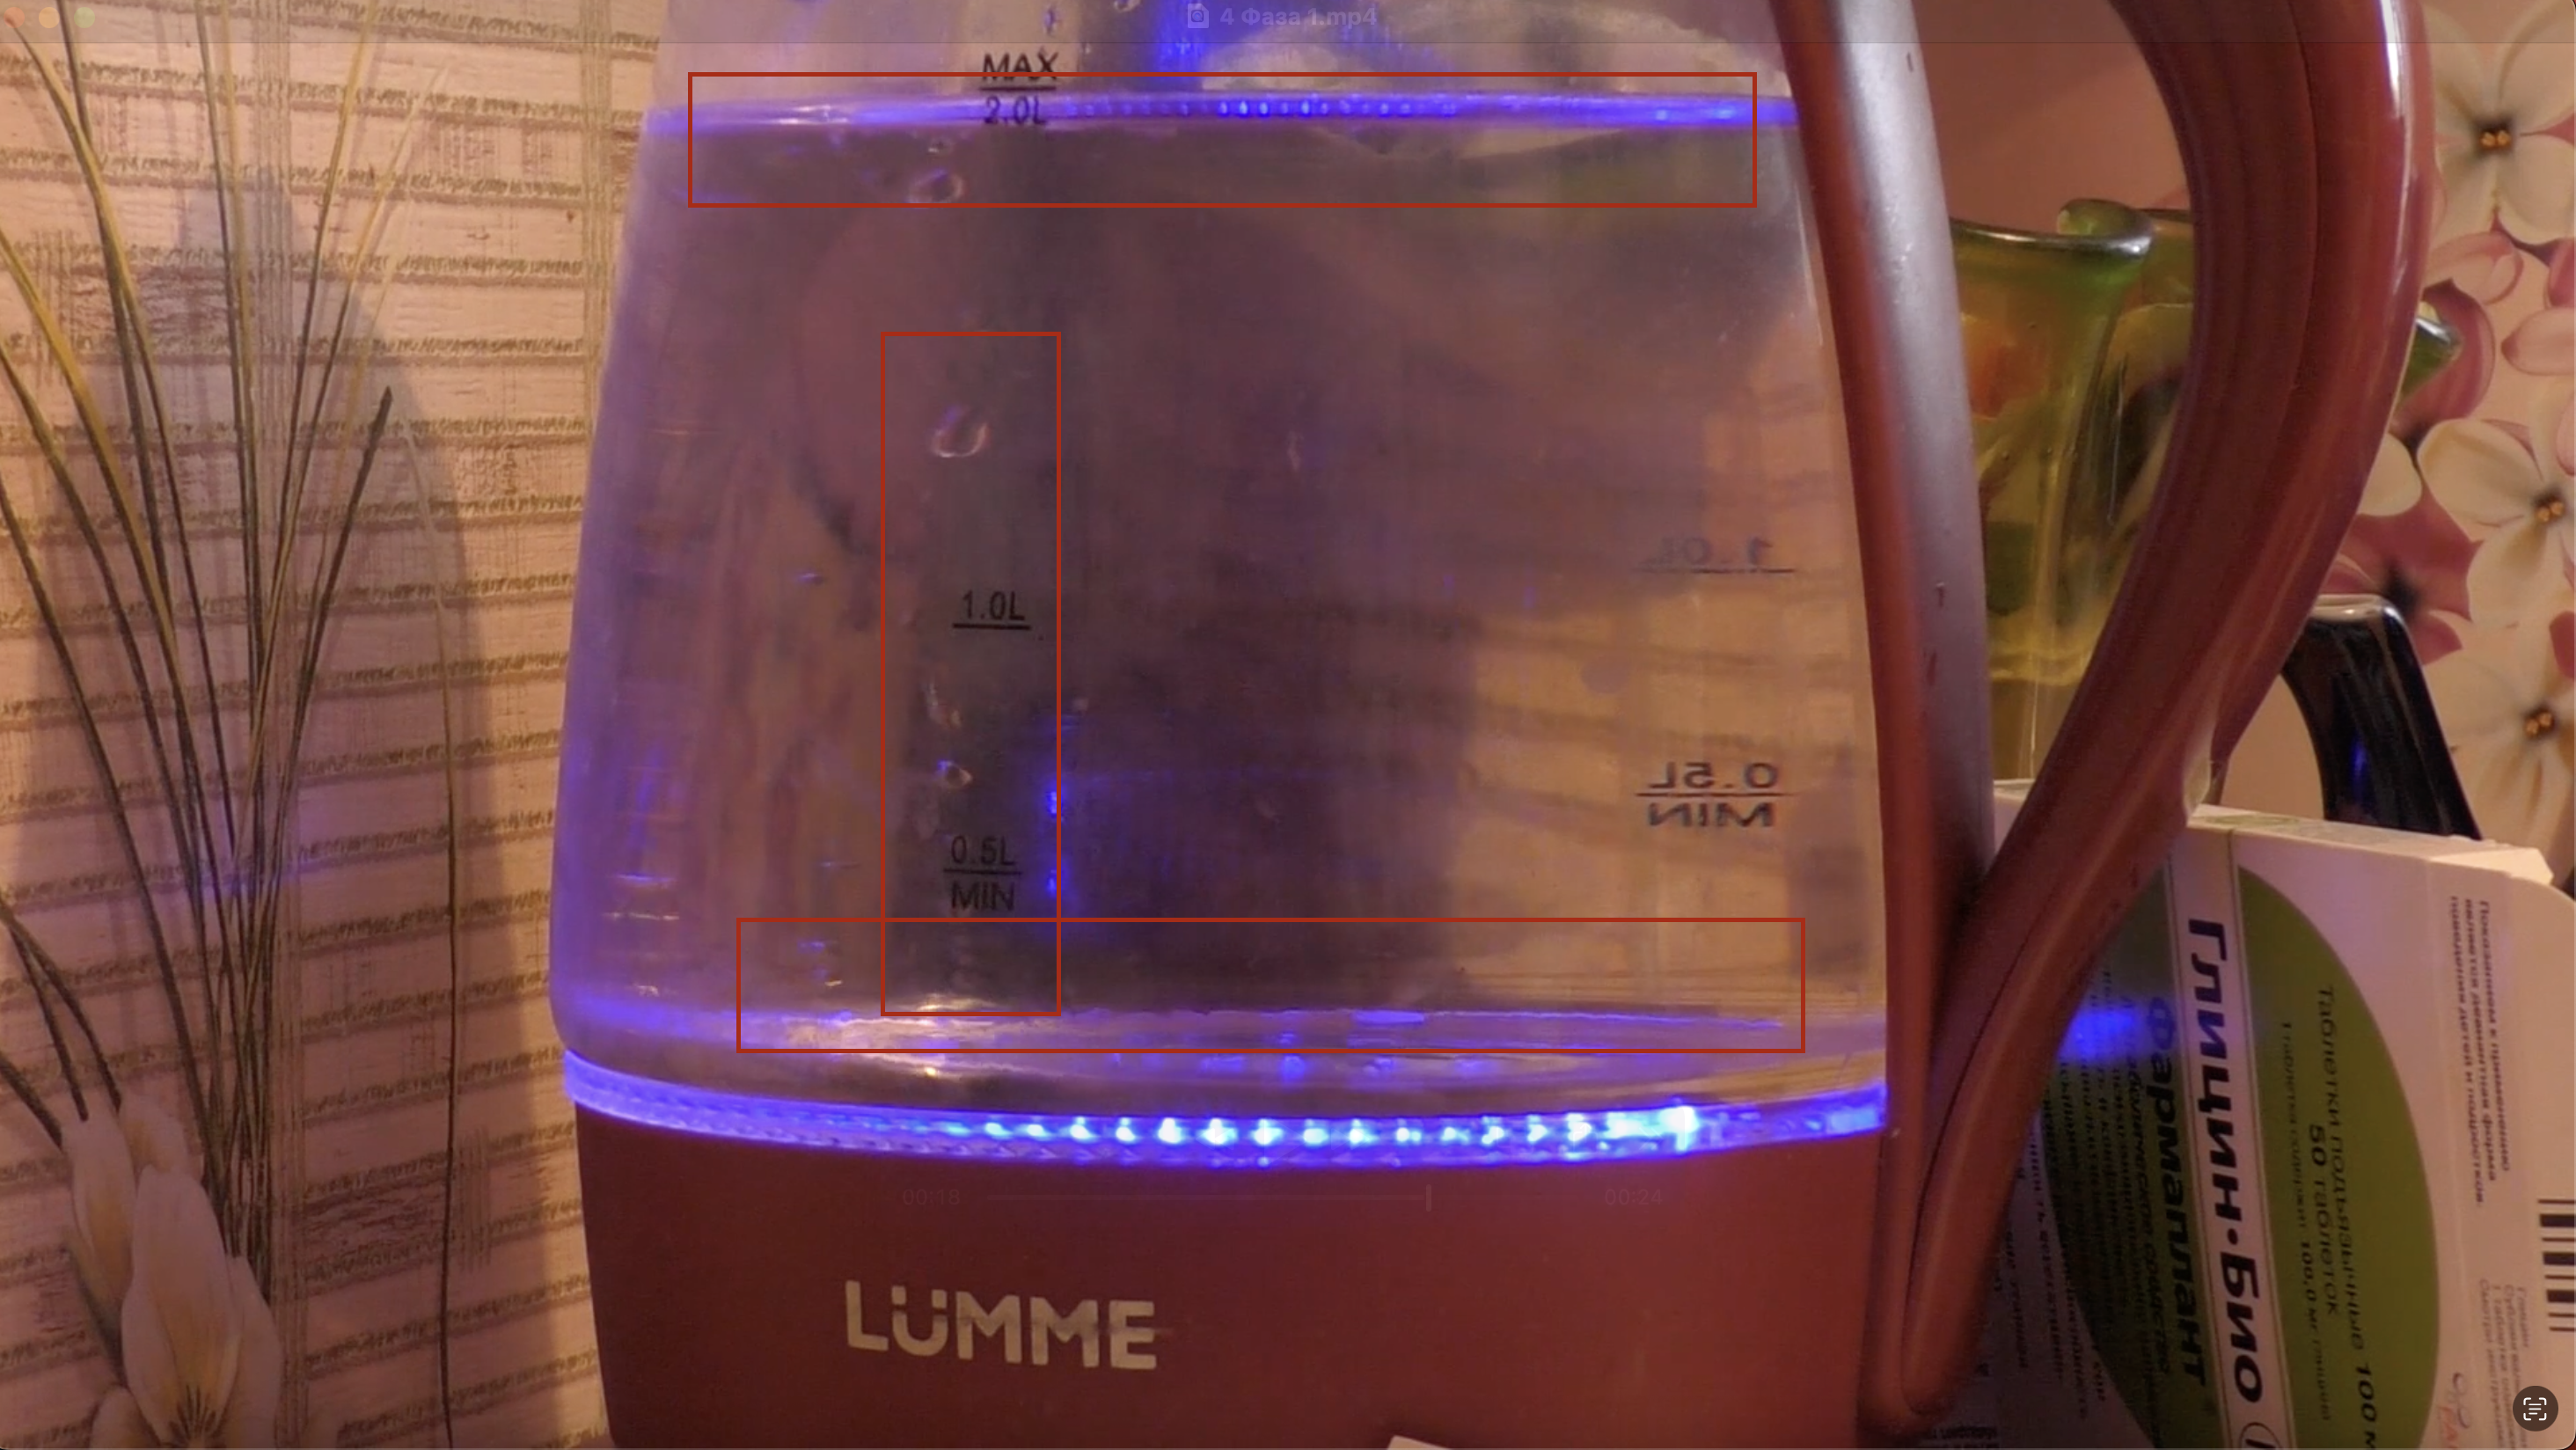
\includegraphics[width=\linewidth]{images/base.png}
        \caption{Базовый кадр}
        \label{fig:base}
    \end{minipage}
\end{figure}

\newpage
\section*{Заключение}
\addcontentsline{toc}{section}{Заключение}
В рамках лабораторной работы была осуществлена визуализация физического процесса кипения воды в чайнике на основе анализа соответствующего видеоролика.
В ходе анализа были выявлены ключевые характеристики динамической и статической составляющих процесса. 
На основе полученных данных была разработана графическая модель с использованием библиотеки Python для визуализации кипения воды.
Для достижения более реалистичного отображения кипения воды применялась техника наложения текстур на изображение. 
Для улучшения точности визуализации можно реализовать более реалистичное движение, форму и прозрачность пузырьков воздуха.
\newpage
\section*{Список литературы}
\addcontentsline{toc}{section}{Список литературы}
\begin{enumerate}
    \item Препарата Ф., Шеймос М., "Вычислительная геометрия: введение"
\end{enumerate}
\end{document}